\documentclass{article}
\usepackage{todonotes}
\usepackage{hyperref}
\usepackage{titlesec}
\titleformat*{\section}{\large}

\title{\textbf{Results for Assignment 1 - Group xx}}
\author{Markus Ruplitsch, Julia Tschuden}


\begin{document}
\maketitle

\section{Task 1}
Information which was deduced from the text: \\
$P(D = 0) = P(H) = 0.95,\\
P(D = 1) = P(A) = 0.04,\\
P(D = 2) = P(C) = 0.01,\\
P(T = 1 | C) = 0.98;   P(T = 0 | C) = 1 - P(T = 1 | C) = 0.02,\\
P(T = 1 | H) = 0.01;   P(T = 0 | H) = 1 - P(T = 1 | H) = 0.99,\\
P(T = 1 | A) = 0.20;   P(T = 0 | A) = 1 - P(T = 1 | A) = 0.80.$

 \begin{table}[!htb]
            \caption{Probability table.}\label{tab1}
            \begin{tabular}{ccccc}
                T/D & H ( D = 0) & A ( D = 1) & C ( D = 2) & p(T$_i$) \\[0.5ex]
                \hline\\[-1.5ex]
                T = 1 & 0.0259 & 0.0011 & 0.0003 & 0.0273 \\[0.5ex]
                T = 0 & 0.9241 &0.0389 & 0.0097 & 0.9727\\[0.5ex]
                \hline
                p($D_i$) & 0.95 & 0.04 & 0.01 & 1\\
            \end{tabular}
        \end{table}
At first calculate the marginal probability.\\
$P(T = 1) = 0.01 * 0.95 + 0.2 * 0.04 + 0.98 * 0.01 = 0.0273$\\
$P(T = 0) = 0.99 * 0.95 + 0.8 * 0.04 + 0.02 * 0.01 = 0.9727$\\\\

Then calculate all joint probabilities.\\
$P(H,T = 1) = P(H) * P(T = 1) = 0.95 * 0.0273 = 0.0259$\\
$P(A,T = 1) = P(A) * P(T = 1) = 0.04 * 0.0273 = 0.0011$\\
$P(C,T = 1) = P(C) * P(T = 1) = 0.01 * 0.0273 = 0.0003$\\\\
$P(H,T = 0) = P(H) * P(T = 0) = 0.95 * 0.9727 = 0.9241$\\
$P(A,T = 0) = P(A) * P(T = 0) = 0.04 * 0.9727 = 0.0389$\\
$P(C,T = 0) = P(C) * P(T = 0) = 0.01 * 0.9727 = 0.0097$\\

\section{Task 2}
Blabla explanation.\\
Blabla.

\section{Task 3}
Blabla explanation.\\
Blabla.

\section{Task 4}
\subsection{Verify conditional mean.}
$E_Y [Y | X = x] = \sum_{n=1}^{N} y_n * p(Y = y_n | X = x)$\\
$ = \sum_{n=1}^{N} y_n * \frac{p(X = x | Y = y_n) * p(Y = y)}{p(X=x)},$\\\\
where $p(X = x)$ is a constant and can be neglected and $p(Y = y_n) = 1$ because of the uniform distribution. Which brings the following equation:\\\\
$ = \sum_{n=1}^{N} y_n * p(X = x | Y = y),$\\\\
however, the equation needs to be normalized. Which is why the formular needs to be divided by $\sum_{n=1}^{N} p(X = x | Y = y)$, which brings following equation:\\\\
$E_Y [Y | X = x] = \frac{\sum_{n=1}^{N} y_n *  p(X = x | Y = y)}{\sum_{n=1}^{N} p(X = x | Y = y)}$



\subsection{Verify MAP.}
$P(Y | X = x) = \frac{P( X = x | Y) * p(Y)}{p(X = x)}$\\
We seek value $y_n \in Y$ that maximises the posterior.\\\\
$\hat{y}_{MAX} = argmax p(Y = y_n | X = x)$\\
$ = argmax \frac{p(X = x | Y = y_n) * p(Y = y_n)}{p(X = x)},$\\\\
where $p(X = x)$ is a constant and can be neglected and $p(Y=y_n) = 1$ because of the uniform distribution. Which brings the following equation:\\\\
$\hat{y}_{MAX} = argmax p(X = x | Y = y_n)$\\

\subsection{Plot results.}
Here the plot containing all result images can be seen. (Sorry for the mess, latex is doing what it wants...) \\
\begin{figure}[h]
  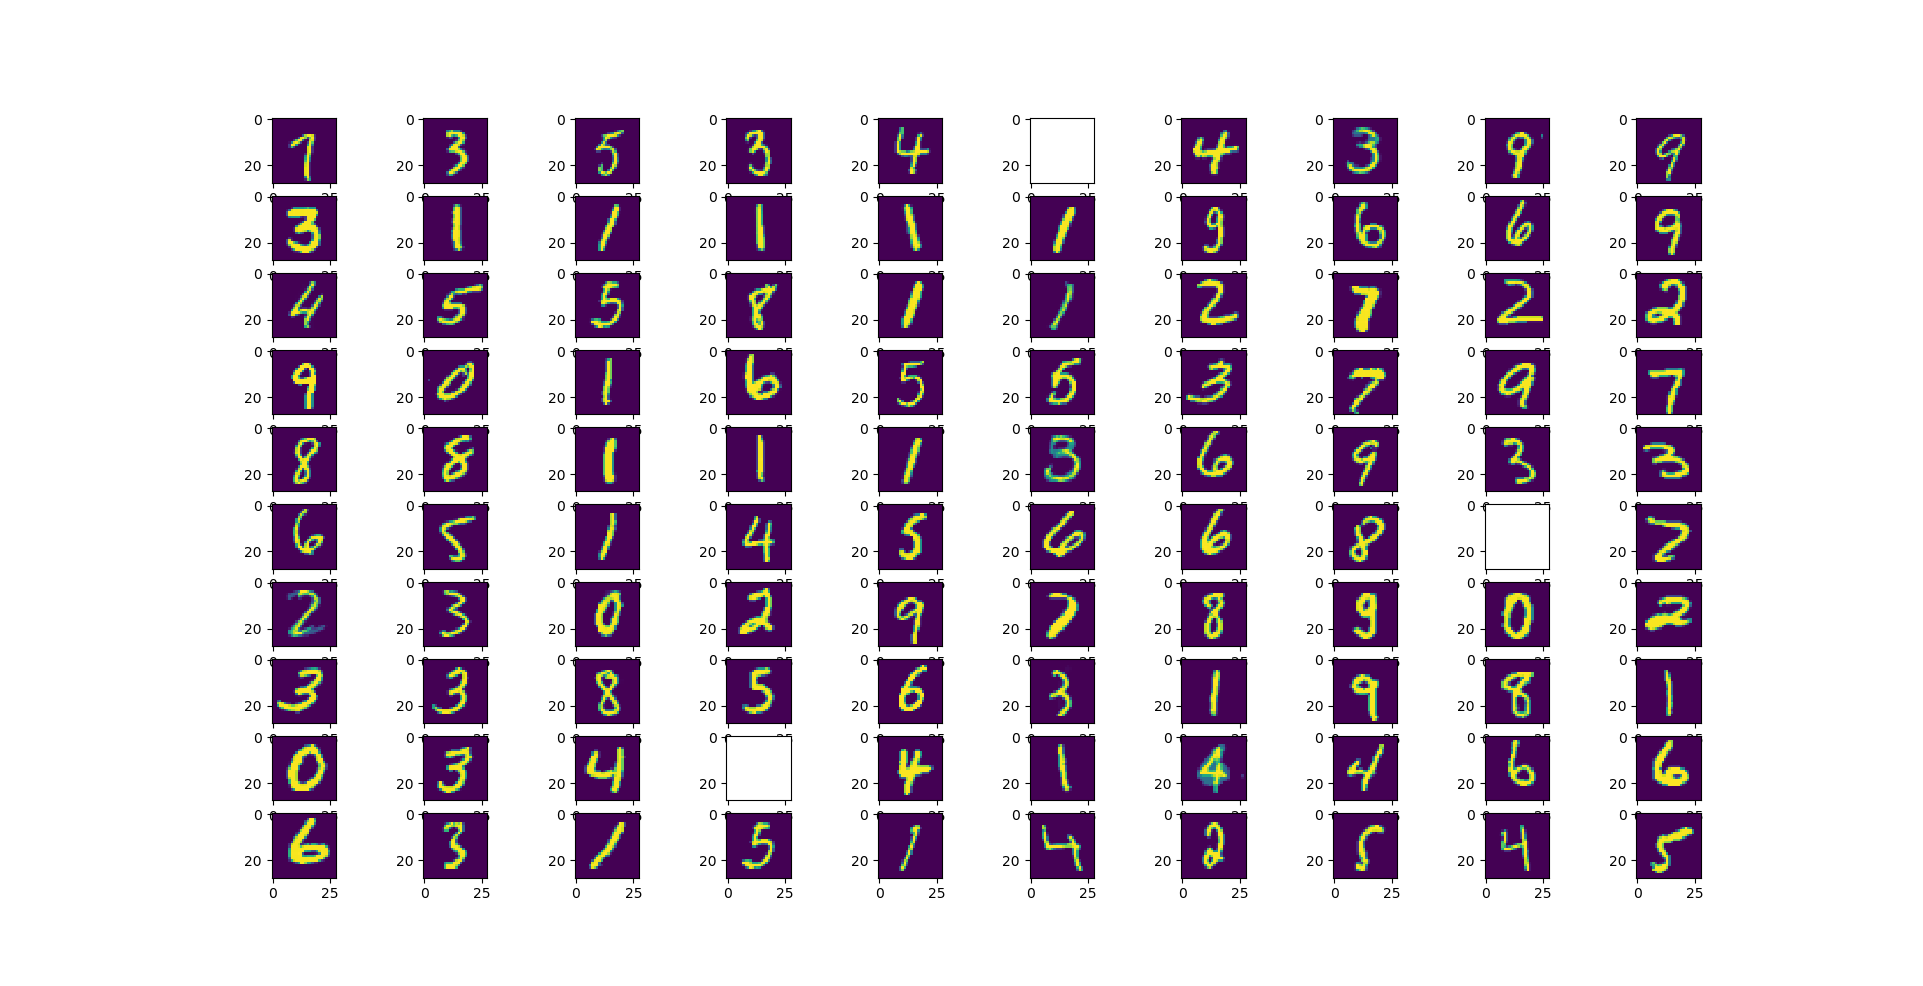
\includegraphics[width=\linewidth]{sigma_025_cm.png}
  \caption{Result of CM algo with sigma 0.25.}
  \label{fig:cm025}
\end{figure}

\begin{figure}[h]
  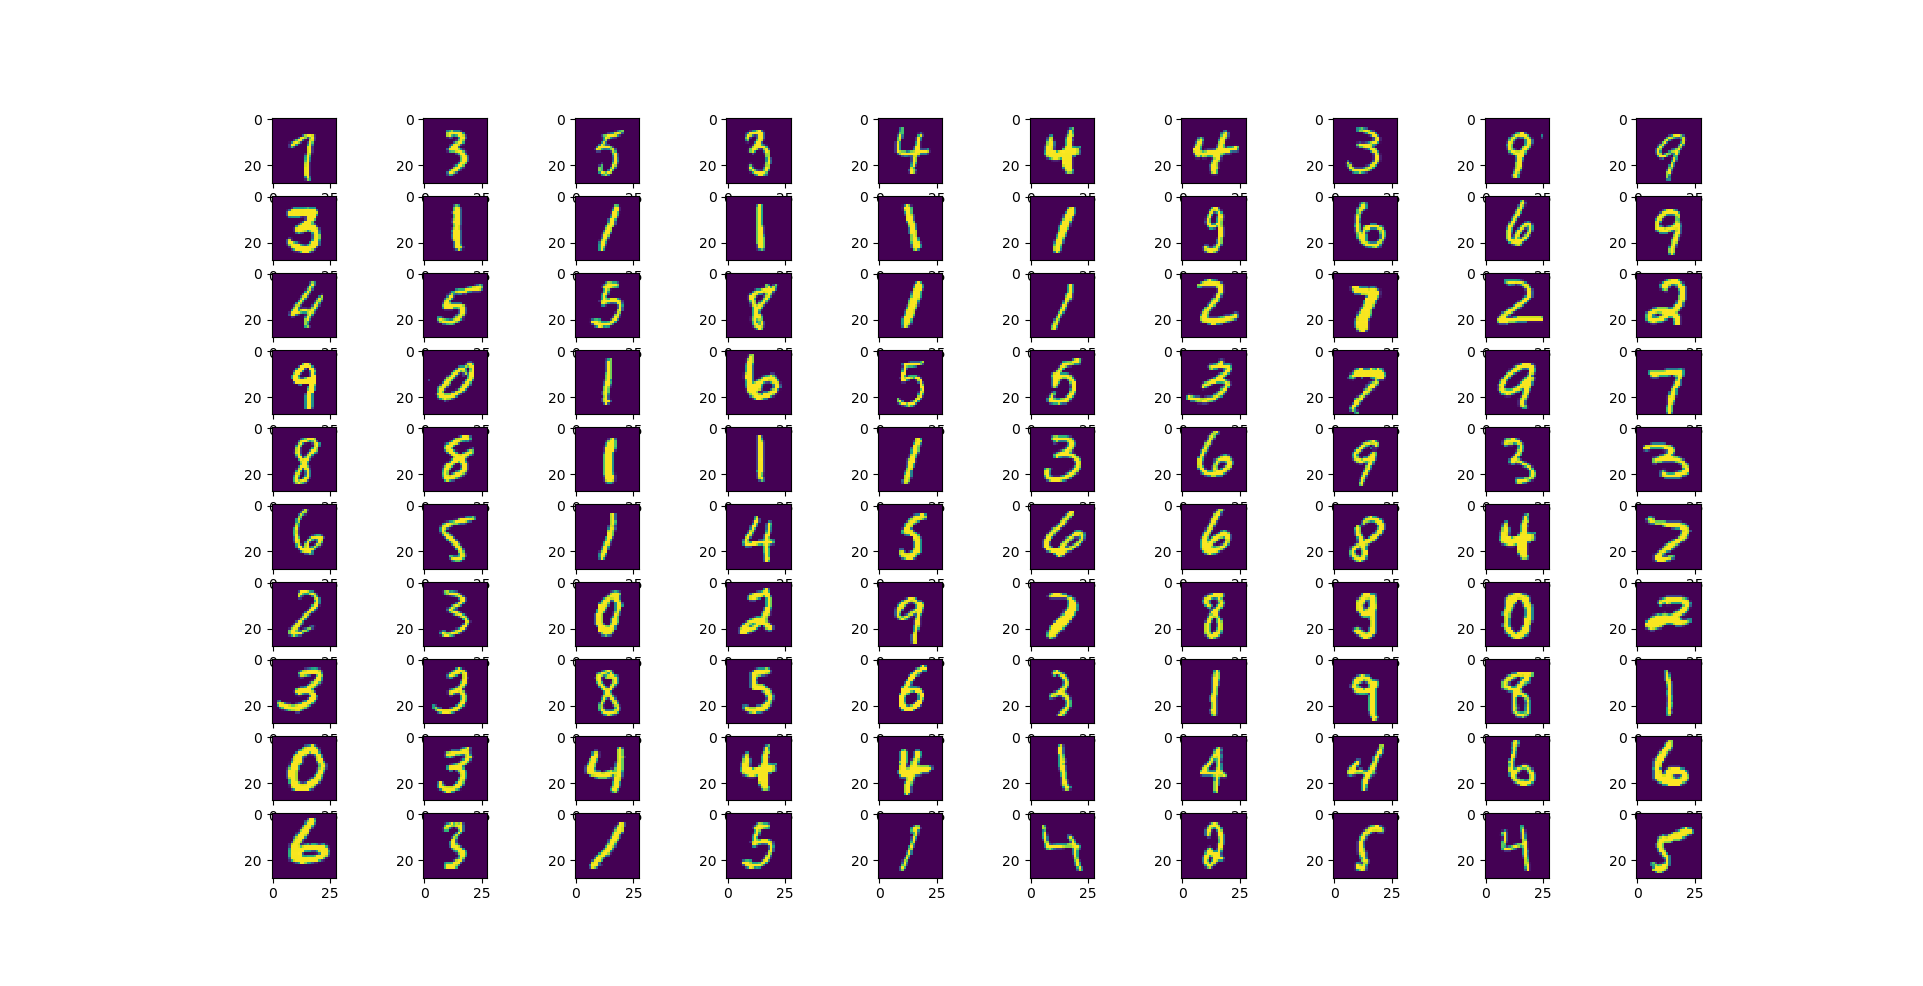
\includegraphics[width=\linewidth]{sigma_025_map.png}
  \caption{Result of MAP algo with sigma 0.25.}
  \label{fig:map025}
\end{figure}

\begin{figure}[h]
  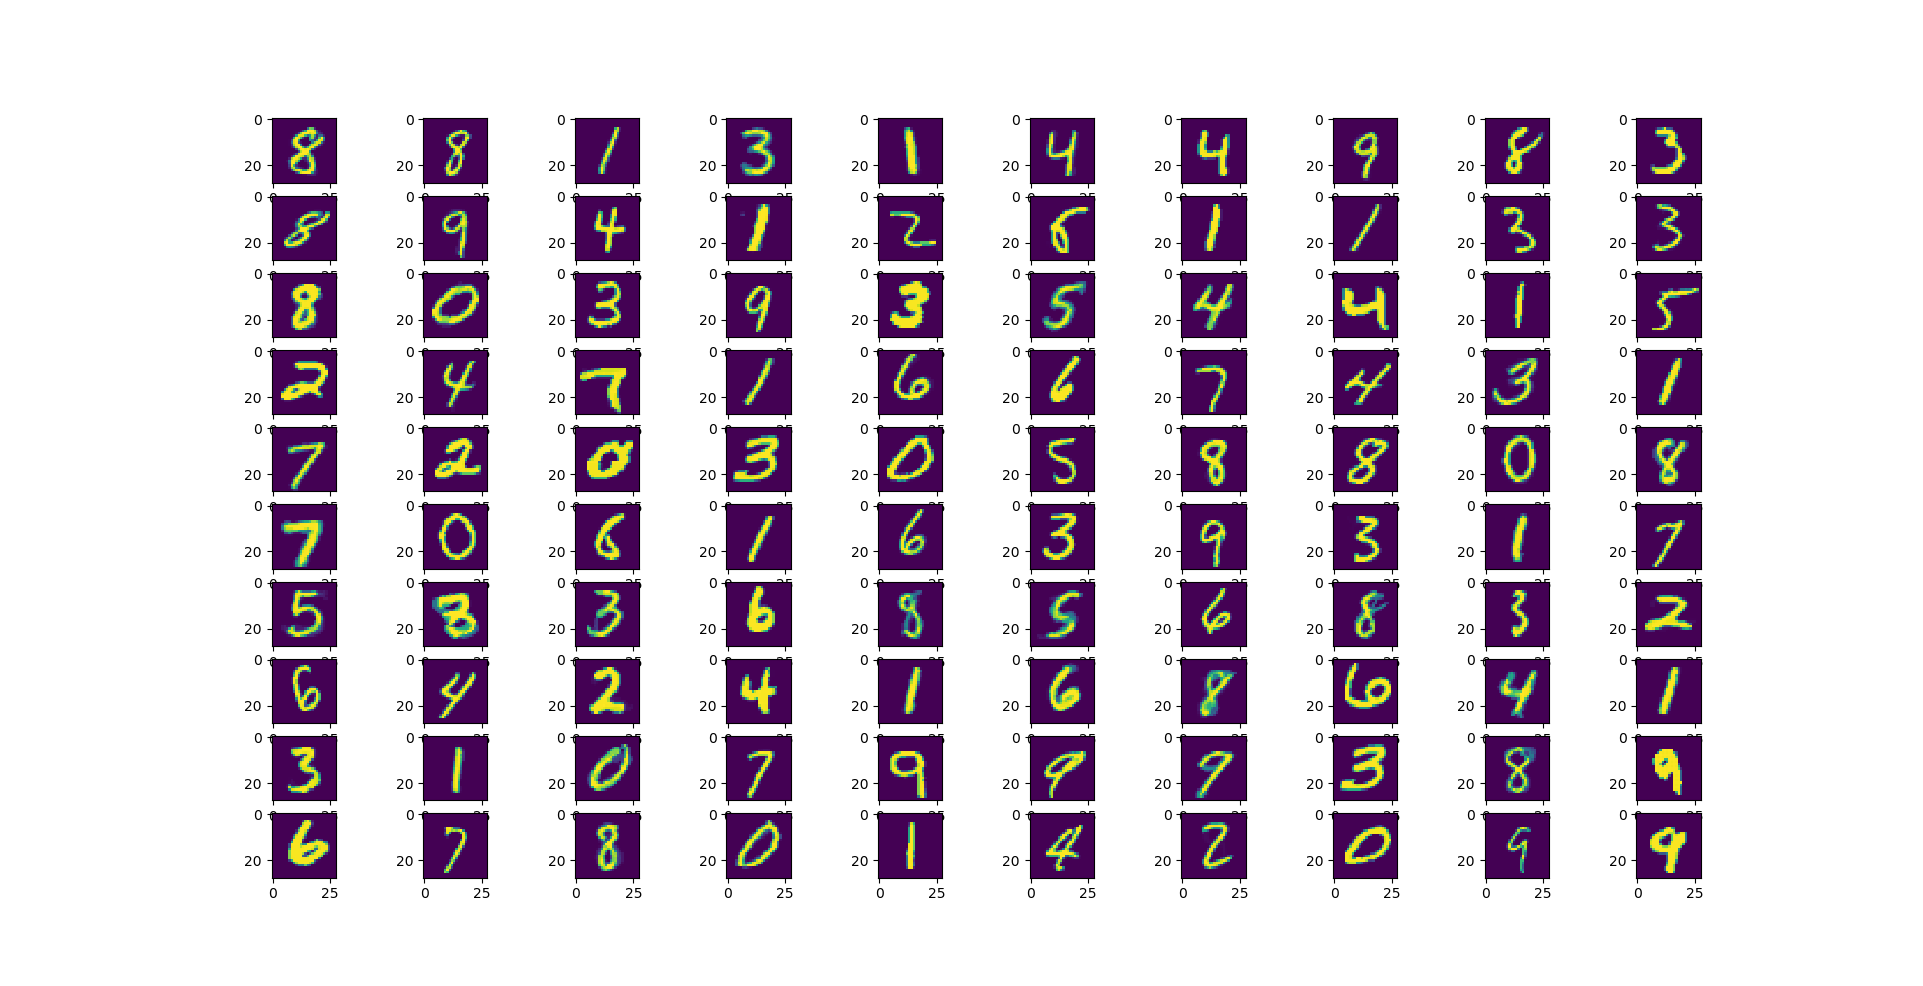
\includegraphics[width=\linewidth]{sigma_050_cm.png}
  \caption{Result of CM algo with sigma 0.50.}
  \label{fig:cm050}
\end{figure}

\begin{figure}[h]
  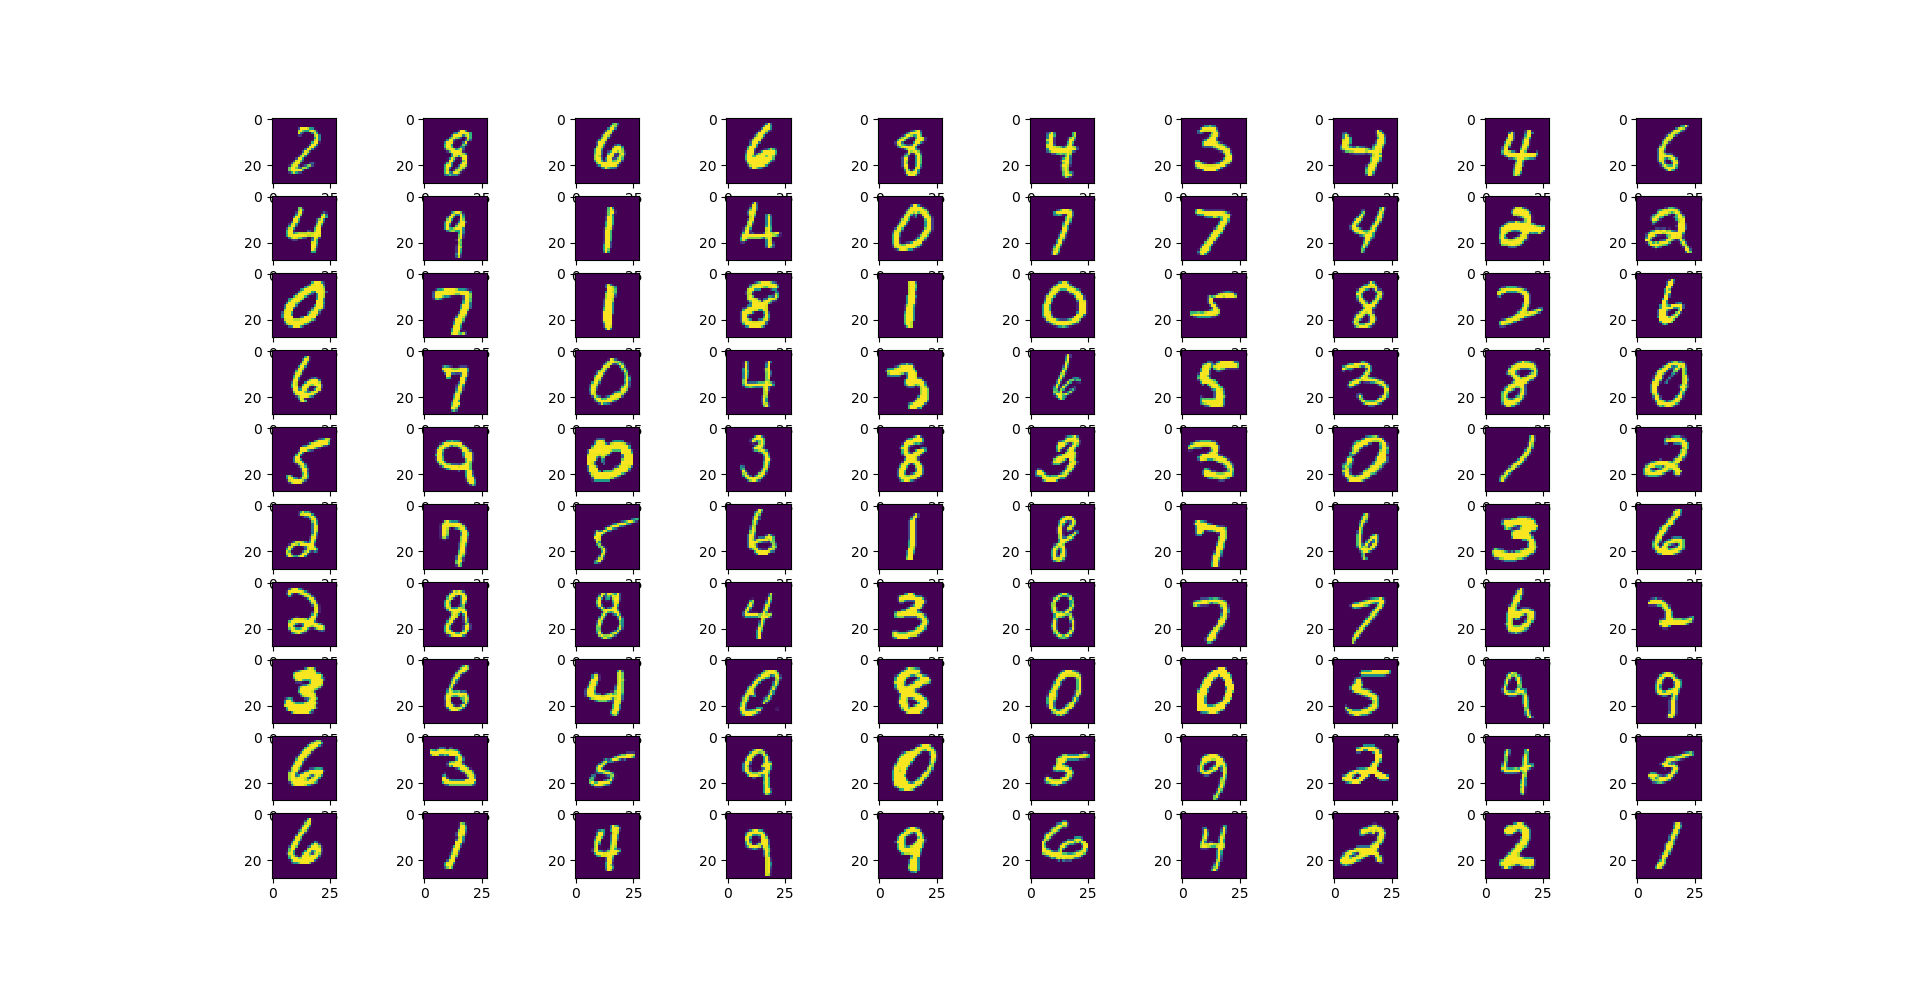
\includegraphics[width=\linewidth]{sigma_050_map.png}
  \caption{Result of MAP algo with sigma 0.50.}
  \label{fig:map050}
\end{figure}

\begin{figure}[h]
  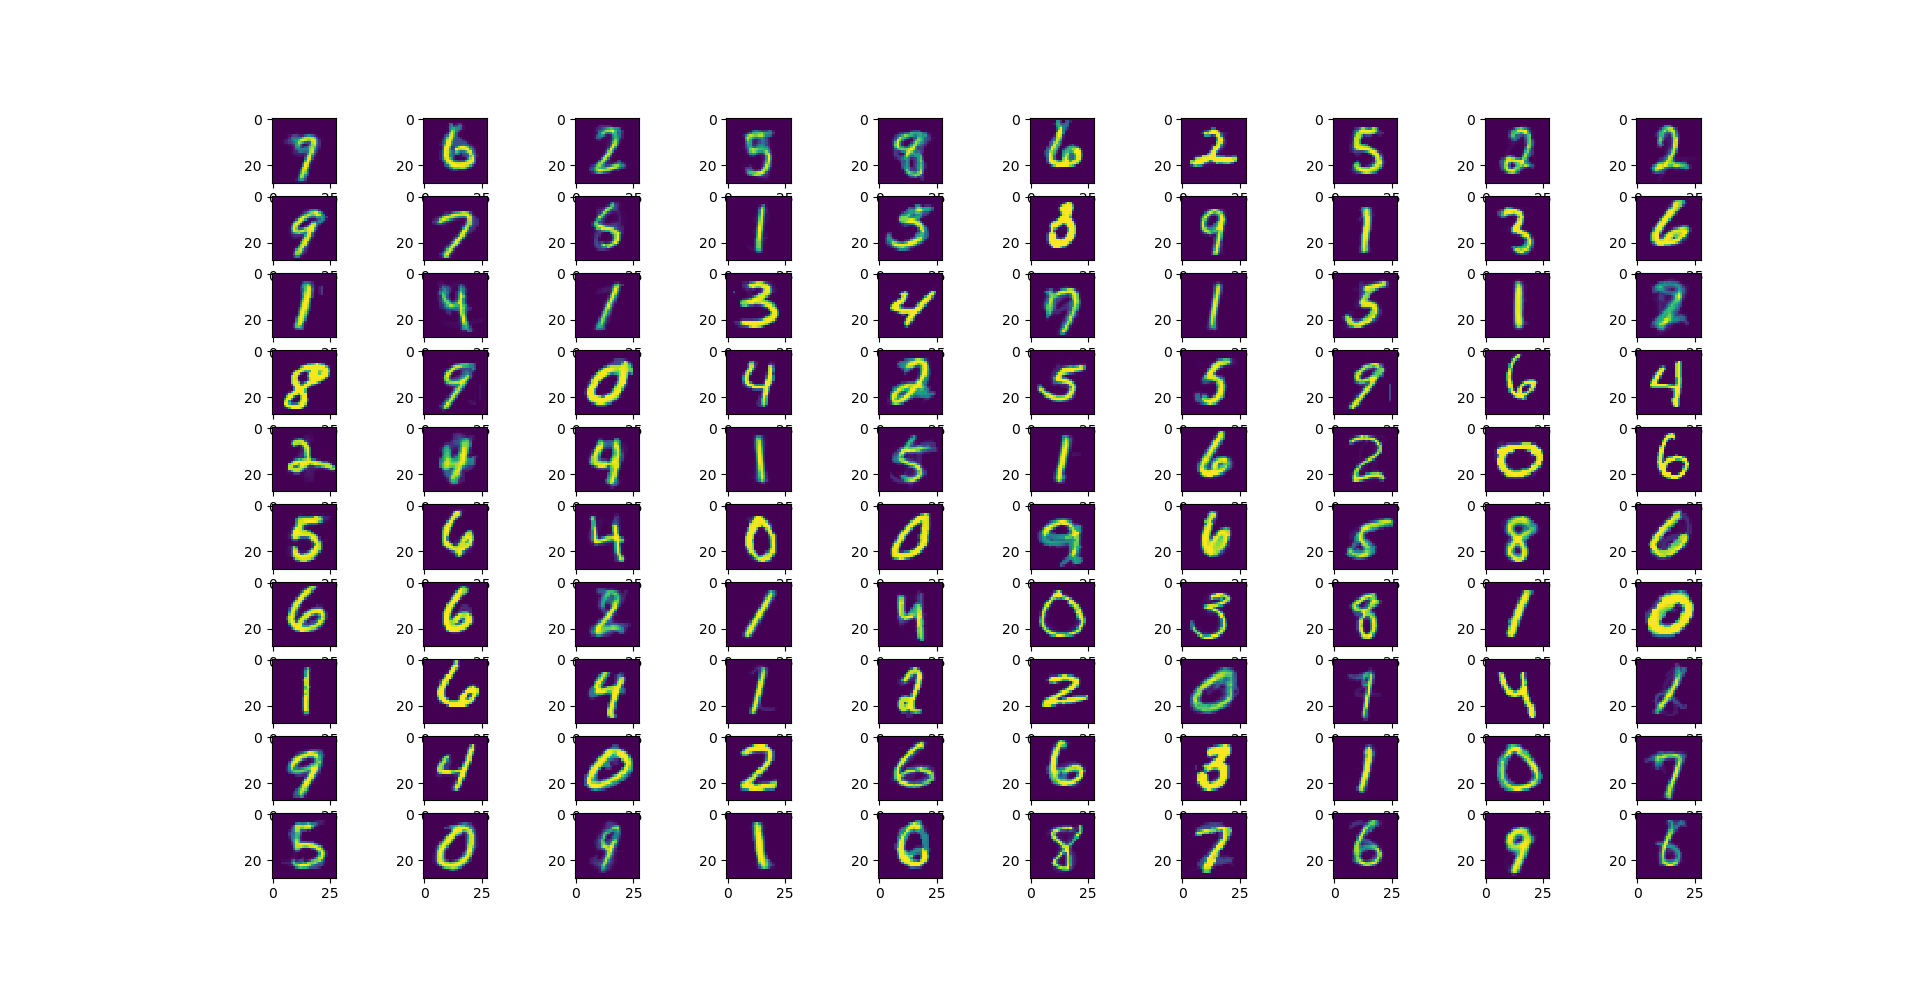
\includegraphics[width=\linewidth]{sigma_100_cm.png}
  \caption{Result of CM algo with sigma 0.50.}
  \label{fig:cm100}
\end{figure}

\begin{figure}[h]
  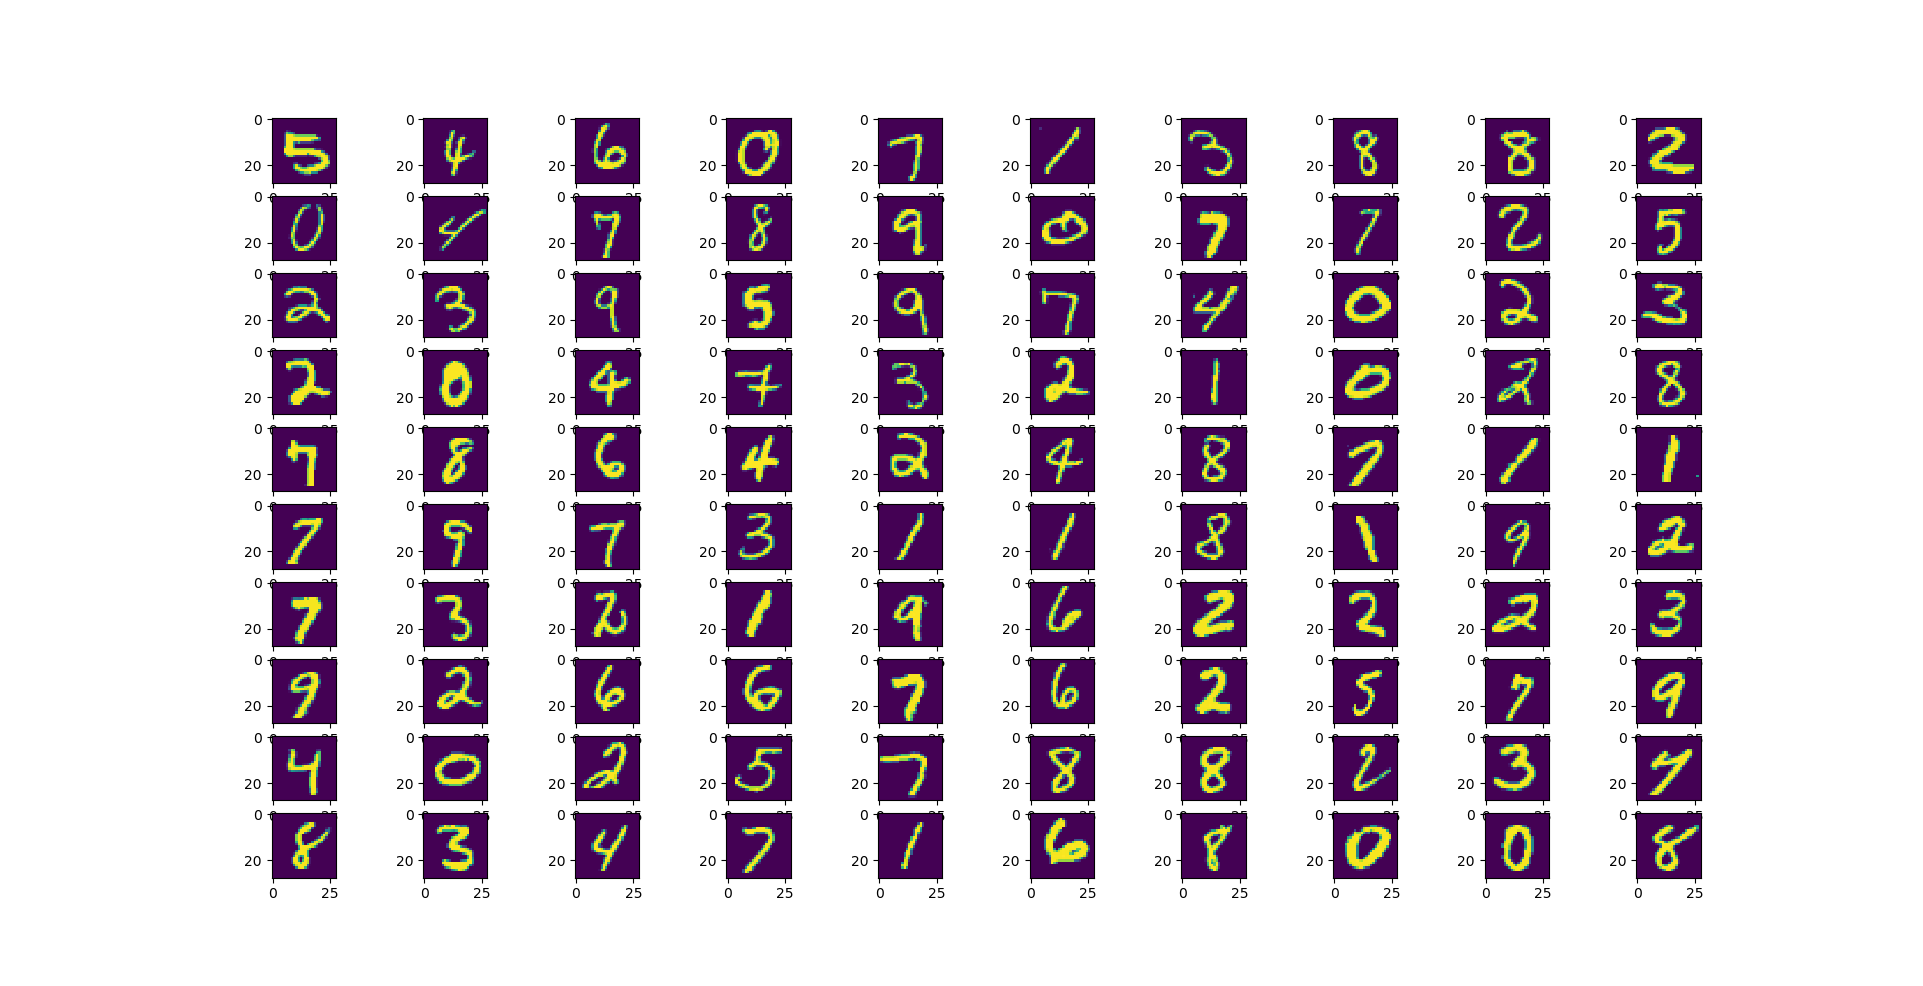
\includegraphics[width=\linewidth]{sigma_100_map.png}
  \caption{Result of MAP algo with sigma 1.0.}
  \label{fig:map100}
\end{figure}

\subsection{Discuss results.}
In our experiments we used three different values for $\sigma: 0.25, 0.5, 1$. The smaller the sigma, the smaller the amount of noise added to the testing images. The bigger the sigma, the bigger the amount of added noise. Generally speaking: the more noise an image has, the harder it is for an algorithm to remove the noise.

\subsubsection{Sigma with 0.25}
As can be seen in figure \ref{fig:cm025} the CM algorithm did a pretty good job at removing the noise. There are only a few images, where the noise was not removed completely (e.g. the 3 at position x=6,y=5, where the algorithm almost made an 8 out of the 3) The MAP algorithm, however, did an excellent job, as can be seen in figure \ref{fig:map025}.

\subsection{Sigma with 0.50}

\end{document}